\documentclass[11pt]{article}
\usepackage[margin=1in]{geometry}
\usepackage{tikz}
\usetikzlibrary{shapes.geometric, arrows.meta, positioning, fit, backgrounds}
\usepackage{booktabs}
\usepackage{xcolor}
\usepackage{adjustbox}

\definecolor{keep}{RGB}{34,139,34}
\definecolor{skip}{RGB}{220,20,60}
\definecolor{neutral}{RGB}{70,130,180}
\definecolor{highlight}{RGB}{255,215,0}

\title{Module 04 Workflow: gnomAD to AlphaGenome Pipeline}
\author{Dormant Site Activation Project}
\date{\today}

\begin{document}

\maketitle

\section{Overview}
This document illustrates the data flow from Module 03 (gnomAD intersection) through Module 04 (deduplication and AlphaGenome scoring) and into downstream analysis. The key innovation is the inclusion of AF=0 variants with known allele number (AN) to capture high-confidence purifying selection signals.

\subsection{What is a Mutation Path?}

A \textbf{mutation path} is a series of single-nucleotide changes that convert a dormant (non-binding) DNA sequence into an active transcription factor binding site.

\textbf{Example: Creating an AP1 binding site (consensus: TGASTCA)}

\begin{center}
\begin{tabular}{lll}
\toprule
\textbf{Step} & \textbf{Sequence} & \textbf{Mutation} \\
\midrule
Start (dormant) & \texttt{AGACTCA} & --- \\
Step 1 & \texttt{TGACTCA} & chr1:1000001 A$>$T \\
Step 2 & \texttt{TGAGTCA} & chr1:1000004 C$>$G \\
Step 3 (active) & \texttt{\textbf{TGAGTCA}} & chr1:1000005 T$>$T (no change) \\
\bottomrule
\end{tabular}
\end{center}

This is \textbf{one mutation path} consisting of 3 steps (2 actual mutations).

\textbf{Key insight:} The genome has $\sim$1.3M sequences that are \emph{close} to AP1 sites---just 1-3 mutations away. Each represents a potential ``dormant site'' that \emph{could} become functional through natural mutations.

\textbf{Why multiple paths to the same variant?}

\textbf{CRITICAL DISTINCTION:} Mutation paths are \textbf{hypothetical trajectories} at the \emph{same genomic location}, not different sequences at different positions.

\textbf{Example:} The genome currently has sequence \texttt{TGACTCA} at chr1:1000001-1000007.

\begin{center}
\begin{tabular}{lp{6cm}l}
\toprule
\textbf{Path} & \textbf{Hypothetical scenario} & \textbf{Mutation needed} \\
\midrule
Path A & ``What if this locus \emph{started} as \texttt{AGA\textcolor{red}{C}TCA} and mutated?'' & chr1:1000001 A$>$T, chr1:1000004 C$>$G \\
Path B & ``What if this locus \emph{already has} \texttt{TGA\textcolor{red}{C}TCA} and mutated?'' & chr1:1000004 C$>$G \\
Path C & ``What if this locus \emph{started} as \texttt{GGA\textcolor{red}{C}TCA} and mutated?'' & chr1:1000001 G$>$T, chr1:1000004 C$>$G \\
\bottomrule
\end{tabular}
\end{center}

\textbf{Key point:} All three paths refer to \textbf{the same genomic coordinates} (chr1:1000001-1000007). They represent different \emph{evolutionary scenarios}, not different genomic locations.

\textbf{Why deduplication is valid:}
\begin{itemize}
    \item AlphaGenome scores \textbf{actual genomic context}: chr1:1000004 C$>$G with its real flanking sequence
    \item The flanking sequence is \textbf{identical} for all three paths (same chr:pos)
    \item The 1MB window is \textbf{identical} for all three paths
    \item AlphaGenome will return \textbf{identical scores} for all three
    \item Therefore: Score once, reuse for all paths containing that variant
\end{itemize}

\textbf{What would NOT be deduplicated:}
\begin{itemize}
    \item chr1:1000004 C$>$G $\leftarrow$ Scored once
    \item chr5:2000004 C$>$G $\leftarrow$ Different location, different flanking sequence, scored separately
    \item chr1:9000004 C$>$G $\leftarrow$ Different location, different flanking sequence, scored separately
\end{itemize}

\section{Pipeline Stages}

\subsection{Path Example: From Modules 00-02}

Before Module 03, we've already computed 6.3M mutation paths from 1.3M dormant sites.

\textbf{Two scenarios to distinguish:}

\textbf{SCENARIO 1: Same genomic location (WILL be deduplicated)}

The genome has \texttt{TGACTCA} at chr1:1000001-1000007. We compute multiple hypothetical paths:

\begin{table}[h!]
\centering
\small
\begin{tabular}{llll}
\toprule
\textbf{Path ID} & \textbf{Hypothetical start} & \textbf{Target} & \textbf{Mutations} \\
\midrule
path\_001 & \texttt{AGACTCA} & \texttt{TGAGTCA} & chr1:1000001 A$>$T, chr1:1000004 C$>$G \\
path\_002 & \texttt{TGACTCA} & \texttt{TGAGTCA} & chr1:1000004 C$>$G \\
path\_003 & \texttt{GGACTCA} & \texttt{TGAGTCA} & chr1:1000001 G$>$T, chr1:1000004 C$>$G \\
\bottomrule
\end{tabular}
\caption{\textcolor{keep}{\textbf{Same genomic locus}} (chr1:1000001-1000007) with different hypothetical evolutionary scenarios. Variant chr1:1000004 C$>$G will be scored \textbf{once} since it has identical context.}
\end{table}

\textbf{SCENARIO 2: Different genomic locations (will NOT be deduplicated)}

The genome has \texttt{TGACTCA} at three \emph{different} chromosomal positions:

\begin{table}[h!]
\centering
\small
\begin{tabular}{lll}
\toprule
\textbf{Genomic location} & \textbf{Current sequence} & \textbf{Mutation needed} \\
\midrule
chr1:1000001-1000007 & \texttt{TGACTCA} & chr1:1000004 C$>$G \\
chr5:2000001-2000007 & \texttt{TGACTCA} & chr5:2000004 C$>$G \\
chr9:8000001-8000007 & \texttt{TGACTCA} & chr9:8000004 C$>$G \\
\bottomrule
\end{tabular}
\caption{\textcolor{skip}{\textbf{Different genomic loci}} with different flanking sequences. Each variant scored \textbf{separately} because AlphaGenome uses 1MB windows centered at different positions.}
\end{table}

\textbf{Module 02 output (Scenario 1):}
\begin{verbatim}
path_id  motif_id  step  chr  pos      ref  alt
path_001 site_123  1     1    1000001  A    T
path_001 site_123  2     1    1000004  C    G    <- Same position
path_002 site_123  1     1    1000004  C    G    <- Same position
path_003 site_123  1     1    1000001  G    T
path_003 site_123  2     1    1000004  C    G    <- Same position
\end{verbatim}

Notice: All paths target the \textbf{same motif\_id (site\_123)} at the \textbf{same genomic coordinates}. Variant \texttt{chr1:1000004 C$>$G} appears 3 times but represents \textbf{one unique genomic context}.

\subsection{Stage 1: Module 03 Output}

\textbf{File:} \texttt{paths\_with\_gnomad.tsv} ($\sim$18M rows)

\begin{table}[h!]
\centering
\small
\begin{tabular}{lllllllll}
\toprule
\textbf{chr} & \textbf{pos} & \textbf{ref} & \textbf{alt} & \textbf{AF} & \textbf{AC} & \textbf{AN} & \textbf{is\_missing} & \textbf{coverage\_conf} \\
\midrule
1 & 1000001 & A & G & 0.0001 & 10 & 100000 & 0 & high \\
1 & 1000002 & C & T & 0.0 & 0 & 80000 & 0 & \textcolor{keep}{\textbf{high}} \\
1 & 1000003 & G & A & 0.0 & 0 & 5000 & 0 & low \\
1 & 1000004 & T & C & 0.0 & 0 & 0 & 1 & \textcolor{skip}{\textbf{missing}} \\
1 & 1000001 & A & G & 0.0001 & 10 & 100000 & 0 & high \\
\bottomrule
\end{tabular}
\caption{Module 03 output contains all mutation steps with gnomAD annotations. Note the duplicate variant (chr1:1000001 A$>$G) appearing in multiple mutation paths.}
\end{table}

\textbf{Key Features:}
\begin{itemize}
    \item Same variants appear in MULTIPLE mutation paths
    \item \texttt{is\_missing=0}: Variant observed in gnomAD (known coverage)
    \item \texttt{is\_missing=1}: Variant not in gnomAD (unknown coverage)
    \item \texttt{coverage\_confidence}: Categories based on AN thresholds
    \begin{itemize}
        \item \texttt{high}: AN $\geq$ 50,000 (well-covered)
        \item \texttt{medium}: AN $\geq$ 10,000 (moderate coverage)
        \item \texttt{low}: AN $>$ 0 but $<$ 10,000 (poor coverage)
        \item \texttt{missing}: No gnomAD record
    \end{itemize}
\end{itemize}

\subsection{Stage 2: Module 04 Step 1 - Filter by Coverage}

\textbf{Operation:} Filter \texttt{is\_missing == 0}

\begin{table}[h!]
\centering
\small
\begin{tabular}{lp{3cm}p{6cm}}
\toprule
\textbf{Action} & \textbf{Variant} & \textbf{Rationale} \\
\midrule
\textcolor{keep}{\textbf{✓ KEEP}} & chr1\_1000001\_A\_G & AF$>$0, AN=100K: existing variation \\
\textcolor{keep}{\textbf{✓ KEEP}} & chr1\_1000002\_C\_T & AF=0, AN=80K: \textbf{strong constraint} \\
\textcolor{keep}{\textbf{✓ KEEP}} & chr1\_1000003\_G\_A & AF=0, AN=5K: weak constraint \\
\textcolor{skip}{\textbf{✗ SKIP}} & chr1\_1000004\_T\_C & is\_missing=1: no gnomAD record \\
\bottomrule
\end{tabular}
\caption{Filtering keeps all variants with known coverage (is\_missing=0), including AF=0 variants which represent potential constraint.}
\end{table}

\subsection{Stage 3: Module 04 Step 2 - Deduplicate}

\textbf{Operation:} Remove duplicates by \texttt{variant\_id} = chr\_pos\_ref\_alt

\textbf{Deduplication logic:}
\begin{verbatim}
variant_id = chr + "_" + genomic_position + "_" + ref + "_" + alt
\end{verbatim}

\textbf{What gets deduplicated:}
\begin{itemize}
    \item \textcolor{keep}{chr1\_1000004\_C\_G} from path\_001 (hypothetical start: AGACTCA)
    \item \textcolor{keep}{chr1\_1000004\_C\_G} from path\_002 (hypothetical start: TGACTCA) $\leftarrow$ \textbf{DUPLICATE}
    \item \textcolor{keep}{chr1\_1000004\_C\_G} from path\_003 (hypothetical start: GGACTCA) $\leftarrow$ \textbf{DUPLICATE}
\end{itemize}

$\Rightarrow$ Keep \textbf{ONE} entry for chr1\_1000004\_C\_G (all have identical genomic context)

\textbf{What does NOT get deduplicated:}
\begin{itemize}
    \item chr1\_1000004\_C\_G (1MB window: chr1:500,004-1,500,004)
    \item chr5\_2000004\_C\_G (1MB window: chr5:1,500,004-2,500,004) $\leftarrow$ \textbf{Different context!}
    \item chr9\_8000004\_C\_G (1MB window: chr9:7,500,004-8,500,004) $\leftarrow$ \textbf{Different context!}
\end{itemize}

$\Rightarrow$ Score \textbf{ALL THREE} separately (different flanking sequences in AlphaGenome's 1MB windows)

\textbf{Result:} \texttt{unique\_variants.tsv} ($\sim$7K--10K rows estimated)

\textbf{Reduction:} 18M mutation steps $\rightarrow$ $\sim$10K unique genomic variants (1,800× compression)

\textbf{Why this is scientifically valid:} AlphaGenome only cares about the \textbf{actual genomic sequence context}, not the hypothetical evolutionary trajectory that might have created it.

\subsection{Stage 4: AlphaGenome API Input}

\textbf{Format:} One API request per unique variant

\begin{verbatim}
{
  "chr": "1",
  "pos": 1000002,
  "ref": "C",
  "alt": "T",
  "assembly": "GRCh38"
}
\end{verbatim}

\textbf{What AlphaGenome Predicts:}

AlphaGenome is a deep learning model trained on ENCODE and Roadmap Epigenomics data. For a given variant, it:

\begin{enumerate}
    \item Extracts \textbf{1MB genomic window} centered on the variant position
    \item Runs the \textbf{reference sequence} through the model $\rightarrow$ Predicts expression for $\sim$1000 cell types
    \item Runs the \textbf{alternate sequence} through the model $\rightarrow$ Predicts expression for $\sim$1000 cell types
    \item Computes \textbf{$\Delta$Expression = Expression(alt) - Expression(ref)} for each cell type
\end{enumerate}

\textbf{Output format:}
\begin{verbatim}
{
  "variant_id": "chr1_1000002_C_T",
  "predictions": {
    "K562": {"ref": 5.2, "alt": 3.8, "delta": -1.4},
    "GM12878": {"ref": 4.1, "alt": 4.3, "delta": 0.2},
    "HepG2": {"ref": 3.5, "alt": 3.4, "delta": -0.1},
    ...  // ~1000 cell types
  }
}
\end{verbatim}

\textbf{Key points:}
\begin{itemize}
    \item \textbf{NOT} actual expression levels (those depend on experimental conditions)
    \item \textbf{PREDICTED} expression \emph{potential} based on DNA sequence alone
    \item Captures regulatory logic: TF binding sites, chromatin accessibility, etc.
    \item $\Delta$Expression measures \textbf{functional impact} of the variant
    \item Positive $\Delta$ = variant increases expression; Negative $\Delta$ = decreases expression
\end{itemize}

\textbf{Why 1MB window?}
\begin{itemize}
    \item Captures long-range regulatory elements (enhancers up to 500kb away)
    \item Includes TAD (topologically associating domain) context
    \item Sufficient for chromatin structure and epigenetic state inference
\end{itemize}

\textbf{Performance:}
\begin{itemize}
    \item Rate: $\sim$1.37 variants/second
    \item Estimated time: $\sim$1.5 hours for 7K variants
\end{itemize}

\textbf{What we use from AlphaGenome output:}
\begin{enumerate}
    \item $|\Delta\text{Expression}|$ = Magnitude of functional impact (absolute value)
    \item Tissue-specific effects: Which cell types show strongest response
    \item Direction: Does variant activate or repress the target gene?
\end{enumerate}

\textbf{Multi-modal AlphaGenome output (STORE ALL FEATURES):}

AlphaGenome returns \textbf{all predictions by default} --- we store everything:

\begin{enumerate}
    \item \textbf{$\Delta$Expression:} Gene expression changes ($\sim$1000 cell types) ← \emph{Primary metric}
    \item \textbf{$\Delta$Chromatin accessibility:} ATAC-seq/DNase-seq signal changes
    \item \textbf{$\Delta$Histone modifications:} H3K27ac (active enhancers), H3K4me3 (promoters), H3K27me3 (repression)
    \item \textbf{$\Delta$TF binding:} Changes in transcription factor occupancy (AP1, CTCF, etc.)
    \item \textbf{$\Delta$3D contacts:} Hi-C contact probability changes (long-range interactions)
\end{enumerate}

\textbf{Why store all features (not just expression):}
\begin{itemize}
    \item \textbf{No extra cost:} AlphaGenome returns all features per query anyway
    \item \textbf{Maximum flexibility:} Discover which features best predict constraint post-hoc
    \item \textbf{Mechanistic insights:} Separate direct effects (TF binding, chromatin) from downstream (expression)
    \item \textbf{Tissue specificity:} Different features may dominate in different contexts
    \item \textbf{Robust validation:} Multi-modal consensus strengthens constraint evidence
    \item \textbf{Future-proof:} Enables exploratory analyses without re-querying API
\end{itemize}

\textbf{Enhanced output format:}
\begin{verbatim}
{
  "variant_id": "chr1_1000002_C_T",
  "expression": {"K562": {"delta": -1.4}, ...},
  "atac": {"K562": {"delta": -0.8}, ...},
  "h3k27ac": {"K562": {"delta": -1.2}, ...},
  "h3k4me3": {"K562": {"delta": 0.1}, ...},
  "tf_binding": {"AP1": {"delta": -2.1}, "CTCF": {"delta": 0.0}, ...},
  "hic_contacts": {"chr1:2000000": {"delta": -0.3}, ...}
}
\end{verbatim}

\textbf{Downstream flexibility:}
\begin{itemize}
    \item Test correlation: AF vs $|\Delta\text{Expression}|$, AF vs $|\Delta\text{ATAC}|$, etc.
    \item Identify strongest constraint signal: Which feature best predicts AF=0?
    \item Multi-modal constraint score: CS = $\sum_i w_i |\Delta\text{Feature}_i| \times -\log_{10}(\text{AF})$
    \item Feature-specific tissue patterns: Is H3K27ac constraint stronger than expression in enhancers?
\end{itemize}

\textbf{Implementation strategy:} Since AlphaGenome returns all features by default, parse and store the complete response for each variant. This requires no additional API calls and provides maximum analytical flexibility for constraint validation.

\subsection{Stage 5: Module 04 Output}

\textbf{File:} \texttt{alphagenome\_scores.tsv}

\textbf{Complete multi-modal output (all AlphaGenome features):}
\begin{table}[h!]
\centering
\adjustbox{max width=\textwidth}{
\begin{tabular}{llllllll}
\toprule
\textbf{variant\_id} & \textbf{AF} & \textbf{AN} & \textbf{cov\_conf} & \textbf{$\Delta$expr} & \textbf{$\Delta$ATAC} & \textbf{$\Delta$H3K27ac} & \textbf{...} \\
\midrule
chr1\_1000001\_A\_G & 0.0001 & 100K & high & -0.23 & -0.15 & -0.31 & ... \\
chr1\_1000002\_C\_T & 0.0 & 80K & high & -1.45 & -0.92 & -1.78 & ... \\
chr1\_1000003\_G\_A & 0.0 & 5K & low & -0.88 & -0.45 & -0.12 & ... \\
\bottomrule
\end{tabular}
}
\caption{Enhanced output: Multiple AlphaGenome features per variant enable flexible downstream validation strategies.}
\end{table}

\textbf{Columns for multi-modal output:}
\begin{itemize}
    \item \textbf{Metadata:} variant\_id, chr, pos, ref, alt, AF, AC, AN, coverage\_confidence
    \item \textbf{Expression:} $\Delta$expr\_[tissue] for $\sim$1000 tissues (primary analysis)
    \item \textbf{Chromatin:} $\Delta$ATAC\_[tissue], $\Delta$DNase\_[tissue]
    \item \textbf{Histones:} $\Delta$H3K27ac\_[tissue], $\Delta$H3K4me3\_[tissue], $\Delta$H3K27me3\_[tissue]
    \item \textbf{TF binding:} $\Delta$TF\_[factor] for relevant TFs (AP1, CTCF, etc.)
    \item \textbf{3D contacts:} $\Delta$HiC\_[bin] for genomic contact frequencies
    \item \textbf{Summary:} max\_abs\_delta\_expr, max\_abs\_delta\_atac, etc. (across tissues)
\end{itemize}

\subsection{Stage 6: Downstream Analysis Options}

\textbf{Flexible filtering decided after seeing empirical AN distribution:}

\begin{table}[h!]
\centering
\begin{tabular}{lp{8cm}}
\toprule
\textbf{Strategy} & \textbf{Filter Criteria} \\
\midrule
Option A & Keep ALL scored variants (no AN filter) \\
Option B & \texttt{coverage\_confidence == 'high'} (AN $\geq$ 50K only) \\
Option C & \texttt{AN >= 10000} (medium+ confidence) \\
Option D & Stratify analysis by \texttt{coverage\_confidence} groups \\
\bottomrule
\end{tabular}
\caption{Post-scoring filtering strategies. Decision made empirically after seeing AN distribution in Module 03 results.}
\end{table}

\section{Constraint Categories}

\begin{table}[h!]
\centering
\begin{tabular}{lp{3cm}p{6cm}}
\toprule
\textbf{Category} & \textbf{Criteria} & \textbf{Interpretation} \\
\midrule
Existing variation & AF $>$ 0 & Common or rare variants in population ($\sim$80\%) \\
\rowcolor{highlight!30}
\textbf{Strong constraint} & AF=0, AN $\geq$ 50K & High-confidence purifying selection ($\sim$10--15\%) \\
Moderate constraint & AF=0, AN $\geq$ 10K & Medium-confidence constraint ($\sim$3--5\%) \\
Weak constraint & AF=0, AN $<$ 10K & Low-confidence or coverage artifact ($\sim$2--5\%) \\
\bottomrule
\end{tabular}
\caption{Classification of variants by allele frequency and coverage. Highlighted row shows key innovation: AF=0 with high AN captures true constraint.}
\end{table}

\section{Key Innovation}

\textbf{Traditional approach:} Exclude all AF=0 variants (cannot distinguish constraint from low coverage)

\textbf{Our approach:} 
\begin{enumerate}
    \item Use AN (allele number) as coverage proxy
    \item Keep AF=0 variants with high AN ($\geq$50K alleles = 25K+ individuals sequenced)
    \item Score all observed variants in AlphaGenome
    \item Filter by coverage confidence in downstream analysis
\end{enumerate}

\textbf{Biological rationale:} If a variant has AF=0 despite being interrogated in 25,000+ individuals, this suggests strong purifying selection against that mutation. These are the \emph{most interesting} variants for understanding regulatory constraint.

\section{Data Flow Summary}

\begin{center}
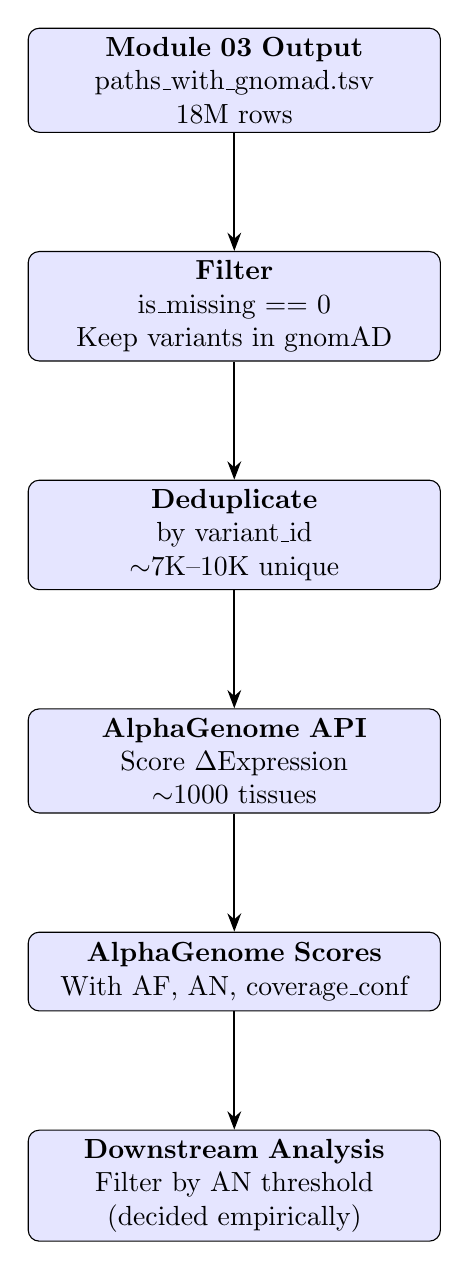
\begin{tikzpicture}[
    node distance=1.5cm,
    box/.style={rectangle, draw, fill=blue!10, text width=5cm, align=center, rounded corners, minimum height=1cm},
    decision/.style={diamond, draw, fill=yellow!20, text width=3cm, align=center, aspect=2},
    arrow/.style={-Stealth, thick}
]

\node[box] (mod3) {\textbf{Module 03 Output}\\paths\_with\_gnomad.tsv\\18M rows};
\node[box, below=of mod3] (filter) {\textbf{Filter}\\is\_missing == 0\\Keep variants in gnomAD};
\node[box, below=of filter] (dedup) {\textbf{Deduplicate}\\by variant\_id\\$\sim$7K--10K unique};
\node[box, below=of dedup] (alpha) {\textbf{AlphaGenome API}\\Score $\Delta$Expression\\$\sim$1000 tissues};
\node[box, below=of alpha] (scores) {\textbf{AlphaGenome Scores}\\With AF, AN, coverage\_conf};
\node[box, below=of scores] (downstream) {\textbf{Downstream Analysis}\\Filter by AN threshold\\(decided empirically)};

\draw[arrow] (mod3) -- (filter);
\draw[arrow] (filter) -- (dedup);
\draw[arrow] (dedup) -- (alpha);
\draw[arrow] (alpha) -- (scores);
\draw[arrow] (scores) -- (downstream);

\end{tikzpicture}
\end{center}

\section{Experimental Validation Strategy}

\subsection{Central Hypothesis}

\textbf{If dormant site activation is constrained by natural selection, then:}

\begin{enumerate}
    \item Variants that \textbf{activate} dormant AP1 sites will have \textbf{stronger functional impact} (larger $|\Delta$Expression|)
    \item These high-impact variants will show \textbf{lower allele frequencies} (AF) due to purifying selection
    \item Variants with \textbf{AF=0 and high AN} represent sites under \textbf{strongest constraint}
\end{enumerate}

\textbf{Expected relationship:} $|\Delta\text{Expression}| \propto \frac{1}{\text{AF}}$ (inversely correlated)

\subsection{Key Comparisons}

\textbf{Standard validation (expression only):}

\begin{table}[h!]
\centering
\begin{tabular}{lp{5cm}p{5cm}}
\toprule
\textbf{Comparison} & \textbf{Prediction} & \textbf{Test} \\
\midrule
AF=0 vs AF$>$0 & AF=0 variants have larger $|\Delta$Expr| & t-test / Mann-Whitney U \\
High vs low AN (within AF=0) & High AN shows stronger constraint signal & Stratified analysis by coverage\_confidence \\
Distance to AP1 motif & Variants closer to motif core show stronger effects & Correlation: distance vs $|\Delta$Expr| \\
Mutation type & CpG transitions may show different patterns & Group by ref$>$alt substitution type \\
\bottomrule
\end{tabular}
\caption{Standard statistical tests using $\Delta$Expression as primary constraint metric.}
\end{table}

\textbf{Enhanced multi-modal validation (if all features available):}

\begin{table}[h!]
\centering
\small
\begin{tabular}{lp{4.5cm}p{5cm}}
\toprule
\textbf{Feature} & \textbf{Hypothesis} & \textbf{Expected AF correlation} \\
\midrule
$\Delta$Expression & Activating AP1 $\rightarrow$ dysregulated genes & \textbf{Strong negative} (r $<$ -0.3) \\
$\Delta$ATAC & Opening chromatin $\rightarrow$ accessibility & Moderate negative (r $<$ -0.2) \\
$\Delta$H3K27ac & Creating active enhancer & \textbf{Strong negative} (r $<$ -0.3) \\
$\Delta$H3K4me3 & Promoter activation & Moderate negative (r $<$ -0.2) \\
$\Delta$TF binding & Direct AP1 binding increase & \textbf{Very strong} (r $<$ -0.4) \\
$\Delta$Hi-C & Altering chromatin loops & Weak negative (r $<$ -0.1) \\
\bottomrule
\end{tabular}
\caption{Multi-modal constraint predictions: Which AlphaGenome features best predict population constraint? Bold = strongest expected signal.}
\end{table}

\textbf{Multi-modal analysis strategies:}
\begin{enumerate}
    \item \textbf{Feature ranking:} Which $\Delta$Feature shows strongest AF correlation?
    \item \textbf{Tissue specificity:} Does constraint vary by cell type/feature?
    \item \textbf{Multi-modal consensus:} Variants with \emph{all} features $>$ threshold
    \item \textbf{Mechanistic dissection:} TF binding vs downstream expression changes
    \item \textbf{Combined score:} Weighted sum across features for constraint ranking
\end{enumerate}

\subsection{Modules 05-07: Downstream Analysis}

\textbf{Module 05: Compute Activation Landscape}
\begin{itemize}
    \item Join AlphaGenome scores back to mutation paths
    \item Calculate per-path functional impact: sum of $|\Delta$Expression| across steps
    \item Identify paths with highest predicted activation potential
    \item Stratify by constraint level (AF=0 high AN vs AF$>$0)
\end{itemize}

\textbf{Module 06: Visualization}
\begin{itemize}
    \item \textbf{Scatter plot:} AF (x-axis, log scale) vs $|\Delta$Expression| (y-axis)
    \begin{itemize}
        \item \textcolor{keep}{Green}: AF=0 with high AN (high-confidence constraint)
        \item \textcolor{neutral}{Blue}: AF$>$0 (existing variation)
        \item Regression line to test inverse correlation
    \end{itemize}
    \item \textbf{Violin plots:} Distribution of $|\Delta$Expression| by AF category
    \item \textbf{Heatmap:} Tissue-specific constraint patterns
\end{itemize}

\textbf{Module 07: Population Statistics}
\begin{itemize}
    \item Calculate enrichment: Are high-impact variants depleted in population?
    \item Test: $\chi^2$ for AF=0 enrichment among top 10\% $|\Delta$Expression| variants
    \item Calculate constraint score: CS = $-\log_{10}(\text{AF} + \epsilon) \times |\Delta\text{Expr}|$
    \item Rank dormant sites by constraint score
\end{itemize}

\subsection{Expected Outcomes}

\textbf{If hypothesis is correct:}
\begin{enumerate}
    \item \textbf{Negative correlation:} Higher $|\Delta$Expression| $\rightarrow$ Lower AF (p $<$ 0.001)
    \item \textbf{AF=0 enrichment:} Top 10\% functional impact variants show $>$30\% AF=0 rate (vs $\sim$15\% baseline)
    \item \textbf{AN matters:} Within AF=0, high AN (50K+) shows stronger $|\Delta$Expression| than low AN
    \item \textbf{Tissue specificity:} Constraint strongest in tissues where AP1 is critical (immune, stress response)
\end{enumerate}

\textbf{If hypothesis is incorrect:}
\begin{itemize}
    \item No correlation between AF and $|\Delta$Expression|
    \item AF=0 variants are random (coverage artifacts, not selection)
    \item High AN provides no additional signal
\end{itemize}

\subsection{Biological Interpretation}

\textbf{Success scenario:} We identify $\sim$100-1000 dormant AP1 sites that are:
\begin{itemize}
    \item Just 1-3 mutations from activation
    \item Under strong purifying selection (AF=0, high AN)
    \item Predicted to have large regulatory impact ($|\Delta$Expr| $>$ 2-fold)
    \item Located in disease-relevant loci (GWAS overlap)
\end{itemize}

\textbf{Applications:}
\begin{enumerate}
    \item \textbf{Therapeutic targets:} Sites that could be activated by genome editing
    \item \textbf{Disease mechanisms:} Rare variants in these paths may cause disease
    \item \textbf{Evolutionary insights:} Regulatory constraint shapes genome evolution
    \item \textbf{Synthetic biology:} Design principles for programmable gene regulation
\end{enumerate}

\end{document}
